\documentclass{report}
\usepackage[T1]{fontenc} % Fontes T1
\usepackage[utf8]{inputenc} % Input UTF8
\usepackage[backend=biber, style=ieee]{biblatex} % para usar bibliografia
\usepackage{csquotes}
\usepackage[portuguese]{babel} %Usar língua portuguesa
\usepackage{blindtext} % Gerar texto automaticamente
\usepackage[printonlyused]{acronym}
\usepackage{hyperref} % para autoref
\usepackage{graphicx}
\usepackage{indentfirst}
\usepackage{float}
%\usepackage{amsmath, amssymb}
%\usepackage{caption}
%\usepackage{geometry}
\usepackage{array}
\usepackage{multirow}

%\usepackage{titlesec}

\usepackage{fancyhdr}

\pagestyle{fancy}  % Ativa o estilo fancyhdr

\lhead{
\includegraphics[width=0.5cm]{code/images/ua.pdf} UA}   % Cabeçalho à esquerda
\chead{Redes de Comunicações I}    % Cabeçalho no centro
\rhead{Grupo 4}    % Cabeçalho à direita

% Formato e espaçamento para os capítulos
%\titleformat{\chapter}[hang]{\huge\bfseries}{\thechapter}{10pt}{\Huge}
%\titlespacing*{\chapter}{0pt}{-20pt}{20pt} 


\bibliography{bibliografia}

\begin{document}
%%
% Definições
%
\def\autores{Fábio Franco, Ricardo Domingues}
\def\empresa{Universidade de Aveiro}
\def\logotipo{ua.pdf}
%
%%%%%% CAPA %%%%%%
%
\begin{titlepage}
    \centering
    {\LARGE {Redes de Comunicações I}}\\
    \vspace{0.5cm}
    {\LARGE Universidade de Aveiro}\\
    \vspace{1.5cm}
    
\includegraphics[width=1.5cm]{code/images/ua.pdf} % Adicione o logo da universidade se necessário
    \vspace{1.5cm}
    
    {\Large \textbf{Departamento de Eletrónica, Telecomunicações e Informática}}\\
    \vspace{0.5cm}
    {\large \textbf{Ano 2024/2025}}\\
    
    \vfill
    
    {\Large \textbf{Report - Fase 1}}\\
    \vspace{0.5cm}
    % \Large \textbf{Fase 1}}\\
    
    \vfill
    
    \vspace{2cm}
    \begin{center}
      \large \textbf{14 de Novembro de 2024}
    \end{center}
    \vspace{0.1cm}
    \begin{center}
    \fbox{\parbox{6cm}{\centering \textbf{P4 - Grupo 4}  \vspace{0.2cm} \\ Fábio Franco (119826) \vspace{0.1cm} \\ Ricardo Domingues (119521) \vspace{0.1cm} }}
    \end{center}
    
\end{titlepage}

\pagenumbering{roman}

%\renewcommand{\contentsname}{Índice}
%\tableofcontents
% \listoftables     % descomentar se necessário
% \listoffigures    % descomentar se necessário

%%%%%%%%%%%%%%%%%%%%%%%%%%%%%%%
\clearpage
\pagenumbering{arabic}

%%%%%%%%%%%%%%%%%%%%%%%%%%%%%%%%
%\chapter{Números Mecanográficos}
\vspace{1.0cm}
\section*{\centerline{Números Mecanográficos}}
Os números mecanográficos utilizados ao longo do projeto são 119826 e 119521, sendo:
\begin{itemize}
    \item $x_1$ -> 1
    \item $x_2$ -> 9
    \item $x_3$ -> 8
    \item $x_4$ -> 2
    \item $x_5$ -> 6
    \item $x_6$ -> 1
    \item $x_7$ -> 9
    \item $x_8$ -> 5
    \item $x_9$ -> 2
    \item $x_{10}$ -> 1
\end{itemize}

\vspace{0.2cm}
Endereços IP utilizados ao longo do projeto:

\begin{table}[h!]
\centering
\begin{tabular}{|c|c|c|}
    \hline
     & \textbf{Calendar Inc} & \textbf{Horoscope Inc} \\ \hline
    \textbf{Public IPv4(sub) Network} & 203.128.191.128/25 & 203.12.59.0/25 \\ \hline
    \textbf{Private IPv4 Network} & 172.26.12.0/23 & 172.22.12.0/23 \\ \hline
    \textbf{Global IPv6 Network} & 2002:A198:BC26::/48 & 2002:A125:BC91::/48 \\ \hline
\end{tabular}
\caption{Endereços IP utilizados}
\label{tab:exemplo}
\end{table}

\newpage
%\clearpage

\section*{\centerline{Public IPv4}}
%\chapter{Public IPv4}
\vspace{0.5cm}
\subsection*{Calendar Inc}

\begin{table}[h!]
\hspace*{-3.0cm}
\centering
%\begin{tabular}{|m{2cm}|m{1,3cm}|m{2,3cm}|m{5cm}|m{2,5cm}|m{1cm}|}
\begin{tabular}{|c|c|c|c|c|c|}
    \hline
    & \textbf{Máscara} & \textbf{Rede} & \textbf{Endereços Disponíveis} & \textbf{Broadcast} & \textbf{Default Gateway} \\ \hline
    NAT/PAT & 30 & 203.128.191.184 & 203.128.191.185 a 203.128.191.187 & --- & --- \\ \hline
    VLAN2 & 28 & 203.128.191.160 & 203.128.191.162 a 203.128.191.174 & 203.128.191.175 & 203.128.191.161\\ \hline
    VLAN4 & 27 & 203.128.191.128 & 203.128.191.130 a 203.128.191.158 & 203.128.191.159 & 203.128.191.129\\ \hline
    VLAN6 & 26 & 203.128.191.192 & 203.128.191.194 a 203.128.191.254 & 203.128.191.255 & 203.128.191.193\\ \hline
    VLAN8 & 29 & 203.128.191.176 & 203.128.191.178 a 203.128.191.182 & 203.128.191.183 & 203.128.191.177\\ \hline
    VLAN12 & 30 & 203.128.191.188 & 203.128.191.190 & 203.128.191.191 & 203.128.191.189\\ \hline
\end{tabular}
\caption{Atribuição do IPv4 Público para Calendar Inc}
\label{tab:exemplo5x6}
\end{table}

Tendo uma rede IP 203.128.191.128 com máscara 25 para poder fazer a atribuição de 50 terminais à VLAN 6 necessitamos de dividir a rede em 2, ficando com 203.128.191.128/26 e 203.128.191.192/26 atribuído à VLAN 6.

Pegando agora na rede 203.128.191.128/26, precisamos de 20 terminais para a VLAN 4, ficando com apenas 32 terminais disponíveis para realizar outras distribuições e obtendo assim 203.128.191.128/27 (escolhida para a VLAN 4) e 203.128.191.160/27. 
De seguida realizamos o mesmo processo com a rede 203.128.191.160/27 e como necessitamos de 12 terminais, subdividimos em 2 ficando com 203.128.191.160/28, que atribuímos à VLAN 2 e 203.128.191.176/28 que fica disponível. 

Seguidamente, voltamos a pegar na rede disponível para divisões, neste caso 203.128.191.176/28 e dividimo-la novamente em 2, ficando com 8 terminais disponíveis em cada delas obtendo, 203.128.191.176/29 atribuido à VLAN 8 e 203.128.191.184/29 disponível para novas distribuições.

Por último, como só é possível fazer distribuições até à máscara 30 pois 2 endereços estão reservados para a rede e o broadcast, deparamo-nos que necessitavamos de 2 terminais livres para o NAT/PAT e 1 para a VLAN 12, sendo atribuídos 203.128.191.184/30 e 203.128.191.188/30 respetivamente uma vez que tínhamos 4 terminais disponíveis em cada uma das redes.

\newpage
\clearpage
\begin{figure}[H]
    \hspace*{-4.0cm}
    \centering
    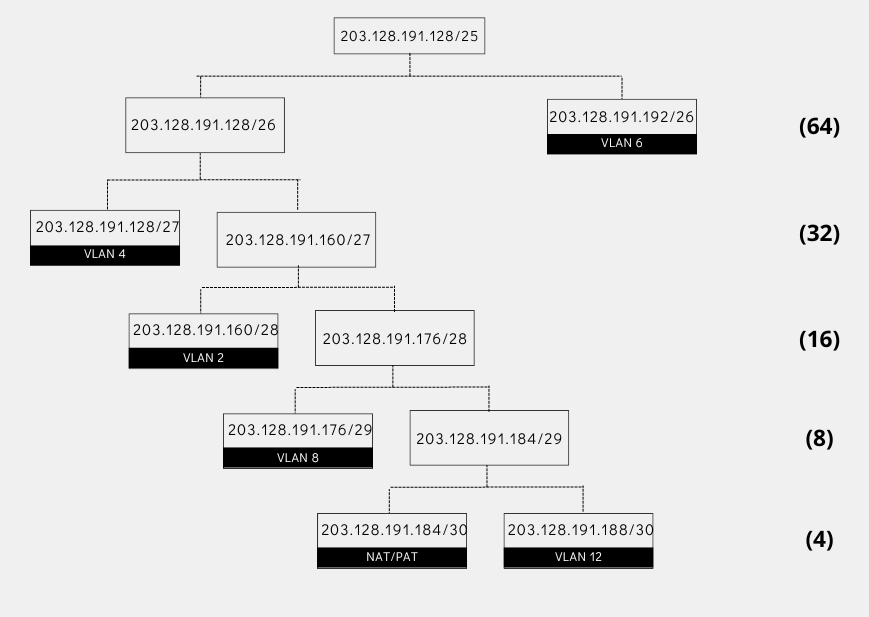
\includegraphics[width=20cm]{code/images/CalendarInc-IPv4 Publico.png}
   % \caption{Legenda da imagem, se desejar} % Opcional
\end{figure}

\newpage
\section*{Horoscope Inc}

\begin{table}[h!]
\hspace*{-3.0cm}
\centering
%\begin{tabular}{|m{2cm}|m{1,3cm}|m{2,3cm}|m{5cm}|m{2,5cm}|m{1cm}|}
\begin{tabular}{|c|c|c|c|c|c|}
    \hline
    & \textbf{Máscara} & \textbf{Rede} & \textbf{Endereços Disponíveis} & \textbf{Broadcast} & \textbf{Default Gateway} \\ \hline
    NAT/PAT & 30 & 203.12.59.56 & 203.12.59.57 a 203.12.59.59 & --- & --- \\ \hline
    VLAN14 & 27 & 203.12.59.0 & 203.12.59.2 a 203.12.59.30 & 203.12.59.31 & 203.12.59.1\\ \hline
    VLAN16 & 27 & 203.12.59.96 & 203.12.59.98 a 203.12.59.126 & 203.12.59.127 & 203.12.59.97\\ \hline
    VLAN18 & 28 & 203.12.59.32 & 203.12.59.34 a 203.12.59.46 & 203.12.59.47 & 203.12.59.33 \\ \hline
    VLAN20 & 28 & 203.12.59.80 & 203.12.59.82 a 203.12.59.94 & 203.12.59.95 & 203.12.59.81\\ \hline
    VLAN22 & 29 & 203.12.59.48 & 203.12.59.50 a 203.12.59.54 & 203.12.59.55 & 203.12.59.49 \\ \hline
    VLAN24 & 30 & 203.12.59.60 & 203.12.59.62 & 203.12.59.63 & 203.12.59.61 \\ \hline
\end{tabular}
\caption{Atribuição do IPv4 Público para Horoscope Inc}
\label{tab:exemplo5x6}
\end{table}

\hspace{4.0cm}

Tendo uma rede IP 203.12.59.0 com máscara 25 para poder fazer a atribuição de 28 terminais à VLAN 14 e de 28 terminais à VLAN 16 necessitamos de dividir a rede em 4, ficando com 203.12.59.32/27, 203.12.59.64/27, 203.12.59.0/27 atribuído à VLAN 14 e 203.12.59.96/27 atribuído à VLAN 16.

Pegando agora na rede 203.12.59.64/27, como precisamos de 10 terminais para a VLAN 20, dividimos em 2, ficando com apenas 16 terminais disponíveis para realizar outras distribuições e obtendo assim 203.12.59.80/28 (escolhida para a VLAN 18) e 203.12.59.64/28.

Do mesmo modo, pegando agora na rede 203.12.59.32/27, precisamos de 13 terminais para a VLAN 18, ficando com apenas 16 terminais disponíveis para realizar outras distribuições e obtendo assim 203.12.59.32/28 (escolhida para a VLAN 18) e 203.12.59.48/28. De seguida realizamos o mesmo processo com a rede 203.12.59.48/28 e como necessitamos de 7 terminais, subdividimos em 2 ficando com 203.12.59.48/29, que atribuímos à VLAN 22 e 203.12.59.56/29 que fica disponível. 

Por último, voltamos a pegar na rede disponível para divisões, neste caso 203.12.59.56/29 e dividimo-la novamente em 2, ficando com 4 terminais disponíveis em cada delas obtendo, 203.12.59.56/30 atribuido ao NAT/PAT e 203.12.59.60/30 atribuido à VLAN 24 (1 terminal necessário).

\newpage
\clearpage
\begin{figure}[H]
    \hspace*{-3.9cm}
    \centering
    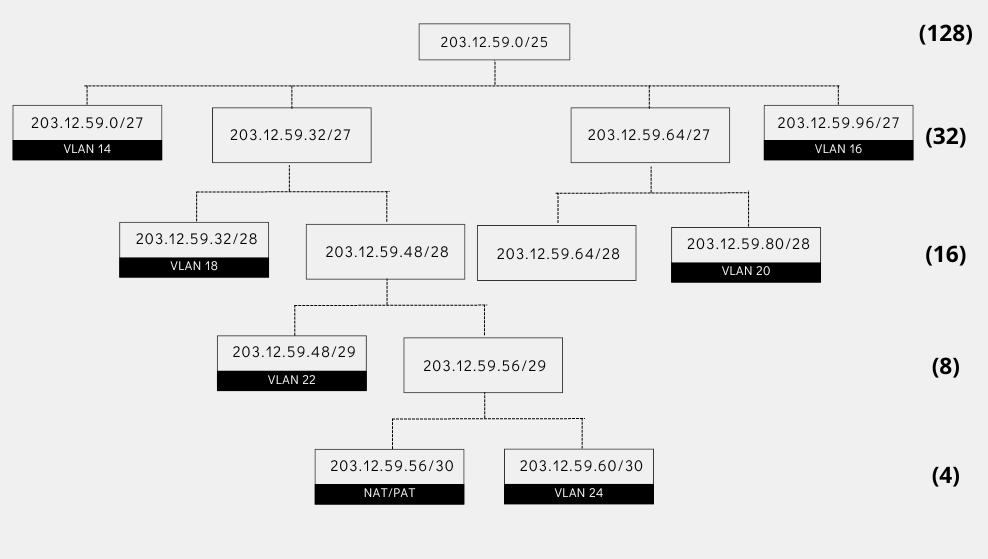
\includegraphics[width=20cm]{code/images/Horoscope Inc - IPv4 Publico.png}
   % \caption{Legenda da imagem, se desejar} % Opcional
\end{figure}

\newpage
\section*{\centerline{Private IPv4}}

\section*{Calendar Inc}

\begin{table}[h!]
\hspace*{-3.0cm}
\centering
%\begin{tabular}{|m{2cm}|m{1,3cm}|m{2,3cm}|m{5cm}|m{2,5cm}|m{1cm}|}
\begin{tabular}{|c|c|c|c|c|c|}
    \hline
    & \textbf{Máscara} & \textbf{Rede} & \textbf{Endereços Disponíveis} & \textbf{Broadcast} & \textbf{Default Gateway} \\ \hline
    VLAN2 & 24 & 172.26.12.0 & 172.26.12.2 a 172.26.12.254 & 172.26.12.255 & 172.26.12.1 \\ \hline
    VLAN4 & 25 & 172.26.13.128 & 172.26.13.130 a 172.26.13.254 & 172.26.13.255 & 172.26.13.129\\ \hline
    VLAN6 & 26 & 172.26.13.0 & 172.26.13.2 a 172.26.13.62 & 172.26.13.63 & 172.26.13.1\\ \hline
    VLAN8 & 27 & 172.26.13.96 & 172.26.13.98 a 172.26.13.126 & 172.26.13.127 & 172.26.13.97\\ \hline
    VLAN12 & --- & --- & --- & --- & --- \\ \hline
    Interconnections & 30 & 172.26.13.64 & 172.26.13.65 a 172.26.13.66 & 172.26.13.67 & --- \\ \hline
\end{tabular}
\caption{Atribuição do IPv4 Privado para Calendar Inc}
\label{tab:exemplo5x6}
\end{table}

\hspace{4.0cm}

Tendo uma rede IP 172.26.12.0 com máscara 23 para poder fazer a atribuição de 200 terminais à VLAN 2 necessitamos de dividir a rede em 2, ficando com 172.26.12.0/24 atribuído à VLAN 2 e 172.26.13.0/24 disponível.

Pegando agora na rede 172.26.13.0/24, precisamos de 110 terminais para a VLAN 4, ficando com apenas 128 terminais disponíveis para realizar outras distribuições e obtendo assim 172.26.13.128/25 (escolhida para a VLAN 4) e 172.26.13.0/25. 

De seguida realizamos o mesmo processo com a rede 172.26.13.0/25 e como necessitamos de 50 terminais, subdividimos em 2 ficando com, 176.26.13.0/26, que atribuímos à VLAN 6 e 172.26.13.64/26 que fica disponível. 

Seguidamente, voltamos a pegar na rede disponível para divisões, neste caso 172.26.13.64/26 e dividimo-la novamente em 2, ficando com 32 terminais disponíveis em cada delas obtendo, 172.26.13.96/27 atribuido à VLAN 8 e 172.26.13.64/27, que fica disponível.

\newpage
\begin{figure}[H]
   \hspace*{-4.0cm}
    \centering
    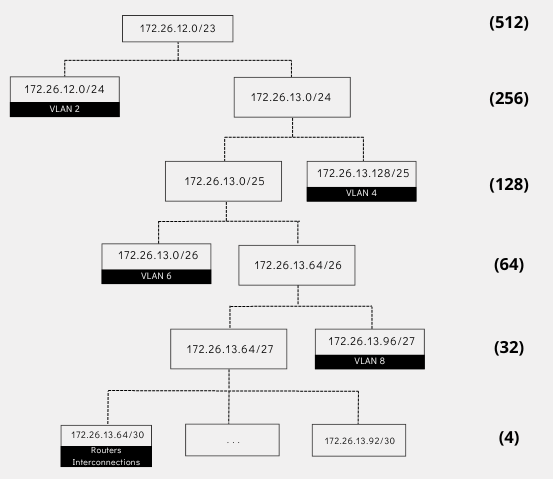
\includegraphics[width=20cm]{code/images/IPv4 Privado - Calendar Inc.png}
   % \caption{Legenda da imagem, se desejar} % Opcional
\end{figure}

\newpage
\clearpage

\section*{Horoscope Inc}

\begin{table}[h!]
\hspace*{-3.0cm}
\centering
%\begin{tabular}{|m{2cm}|m{1,3cm}|m{2,3cm}|m{5cm}|m{2,5cm}|m{1cm}|}
\begin{tabular}{|c|c|c|c|c|c|}
    \hline
    & \textbf{Máscara} & \textbf{Rede} & \textbf{Endereços Disponíveis} & \textbf{Broadcast} & \textbf{Default Gateway} \\ \hline
    VLAN14 & 27 & 172.22.13.64 & 172.22.13.66 a 172.22.13.94 & 172.22.13.95 & 172.22.13.65 \\ \hline
    VLAN16 & 26 & 172.22.13.192 & 172.22.13.194 a 172.22.13.254 & 172.22.13.255 & 172.22.13.193 \\ \hline
    VLAN18 & 26 & 172.22.13.0 & 172.22.13.2 a 172.22.13.62 & 172.22.13.63 & 172.22.13.1 \\ \hline
    VLAN20 & 28 & 172.22.13.96 & 172.22.13.98 a 172.22.13.110 & 172.22.13.111 & 172.22.13.97 \\ \hline
    VLAN22 & 24 & 172.22.12.0 & 172.22.12.2 a 172.22.12.254 & 172.22.12.255 & 172.22.12.1 \\ \hline
    VLAN24 & --- & --- & --- & --- & --- \\ \hline
    Interconnections & 30 & 172.22.13.112 & 172.22.13.113 a 172.22.13.114 & 172.22.13.115 & --- \\ \hline
\end{tabular}
\caption{Atribuição do IPv4 Privado para Horoscope Inc}
\label{tab:exemplo5x6}
\end{table}

Tendo uma rede IP 172.22.12.0 com máscara 23 para poder fazer a atribuição de 155 terminais à VLAN 22 necessitamos de dividir a rede em 2, ficando com 172.22.12.0/24 atribuído à VLAN 22 e 172.22.13.0/24 disponível.

Pegando agora na rede 172.22.13.0/24, precisamos de 57 terminais para a VLAN 18 e 55  terminais para a VLAN 16, ficando com apenas 64 terminais disponíveis para realizar outras distribuições e obtendo assim 172.22.13.0/26 (escolhida para a VLAN 18), 172.22.13.192/26 (para a vlan 16) e 172.22.13.64/26 e 172.22.13.128/26 disponiveis.

De seguida realizamos o mesmo processo com a rede 172.22.13.64/26 e como necessitamos de 25 terminais, subdividimos em 2 ficando com, 172.22.13.64/27, que atribuímos à VLAN 14 e 172.22.13.96/27 que fica disponível. 

Seguidamente, voltamos a pegar na rede disponível para divisões, neste caso 172.22.13.96/27 e dividimo-la novamente em 2, ficando com 16 terminais disponíveis em cada delas obtendo, 172.22.13.96/28 atribuido à VLAN 20 e 172.22.13.96/28, que fica disponível.

\newpage
\begin{figure}[H]
    \hspace*{-4.0cm}
    \centering
    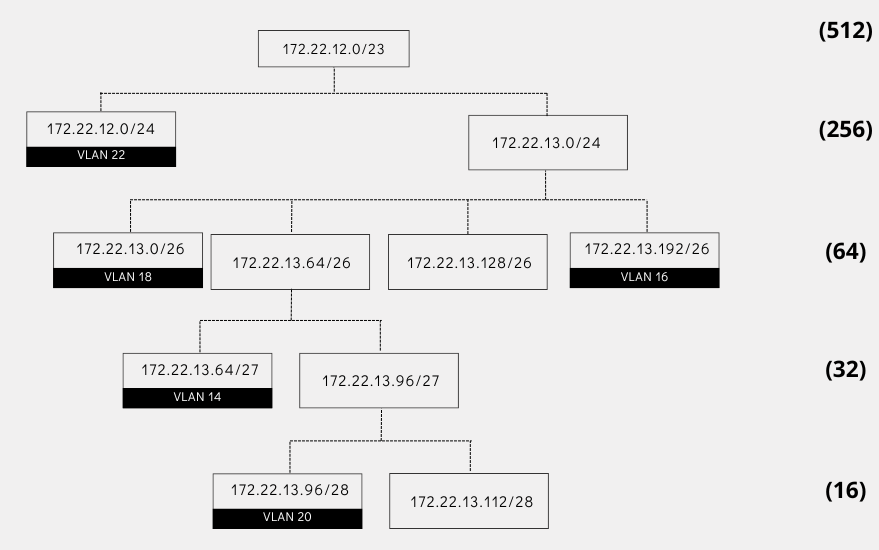
\includegraphics[width=20cm]{code/images/Horoscope Inc - IPv4 Privado.png}
   % \caption{Legenda da imagem, se desejar} % Opcional
\end{figure}

\newpage
\clearpage

\section*{\centerline{Global IPv6}}

\section*{Calendar Inc}

\begin{table}[h!]
    \hspace*{-4.0cm}
    \centering
    \setlength{\tabcolsep}{2pt} % Reduz o espaçamento entre colunas
    \renewcommand{\arraystretch}{1.3} % Aumenta o espaçamento entre linhas
    \begin{tabular}{|c|c|c|c|c|c|} % Reduz a largura do campo Endereços Disponíveis
        \hline
        \textbf{Interface} & \textbf{Rede Interface} & \textbf{VLAN} & \textbf{Rede VLAN} & \textbf{Endereços Disponíveis} & \textbf{Default Gateway} \\ \hline
        
        \multirow{2}{*}{R2} & \multirow{2}{*}{\textbf{P}::/56} & 6 & \textbf{P}:6::/64 & \textbf{P}:6::2/64 a \textbf{P}:6:FFFF:FFFF:FFFF:FFFF/64 & \textbf{P}:6::1/64 \\ \cline{3-6}   
         & & 8 & \textbf{P}:8::/64 & \textbf{P}:8::2/64 a \textbf{P}:8:FFFF:FFFF:FFFF:FFFF/64 & \textbf{P}:8::1/64 \\ \cline{3-6} \hline

         R2 (f1/1) & \textbf{P}::1/126 & --- & --- & --- & --- \\ \hline

         ESW2 (f0/0) & \textbf{P}::2/126 & --- & --- & --- & --- \\ \hline
         
        \multirow{3}{*}{ESW2} & \multirow{3}{*}{\textbf{P}:100::/56} & 2 & \textbf{P}:102::/64 & \textbf{P}:102::2/64 a \textbf{P}:102:FFFF:FFFF:FFFF:FFFF/64 & \textbf{P}:102::1/64 \\ \cline{3-6} 
         & & 4 & \textbf{P}:104::/64 & \textbf{P}:104::2/64 a \textbf{P}:104:FFFF:FFFF:FFFF:FFFF/64 & \textbf{P}:104::1/64 \\ \cline{3-6}   
         & & 12 & \textbf{P}:10C::/64 & \textbf{P}:10C::2/64 a \textbf{P}:10C:FFFF:FFFF:FFFF:FFFF/64 & \textbf{P}:10C::1/64 \\ \hline

    \end{tabular}
    \textbf{Prefix (P):}
    2002:A198:BC26
    \caption{Atribuição do IPv6 Global para Calendar Inc}
\end{table}

Tendo a rede IP 2002:A198:BC26::/48, dividiu-se arbitráriamente por 2 redes IP com máscara /56, sendo estas: 
\begin{itemize}
    \item 2002:A198:BC26::/56;
    \item 2002:A198:BC26:100::/56; 
\end{itemize}

Posteriormente pegou-se na rede 2002:A198:BC26::/56 e dividimo-la em 2, atribuido o endereço 2002:A128:BC26:6::/64 à VLAN 6 e o 2002:A198:BC26:8::/64 à VLAN 8, ambas arbitrárias.

De seguida, e obtida a partir da rede 2002:A198:BC26::/48, obtivemos as seguintes sub-redes para a comunicação entre o Router 2 e o ESW 2:
\begin{itemize}
    \item 2002:A198:BC26::1/126;
    \item 2002:A198:BC26::2/126.
\end{itemize}

Por fim pegamos na rede 2002:A198:BC26:100::/56 e subdividimo-la em 3, atribuindo 2002:A198:BC26:102::/64 à VLAN 2, 2002:A198:BC26:104::/64 à VLAN 4 e 2002:A198:BC26:10C::/64 à VLAN 12.

\newpage
\begin{figure}[H]
    \hspace*{-4.0cm}
    \centering
    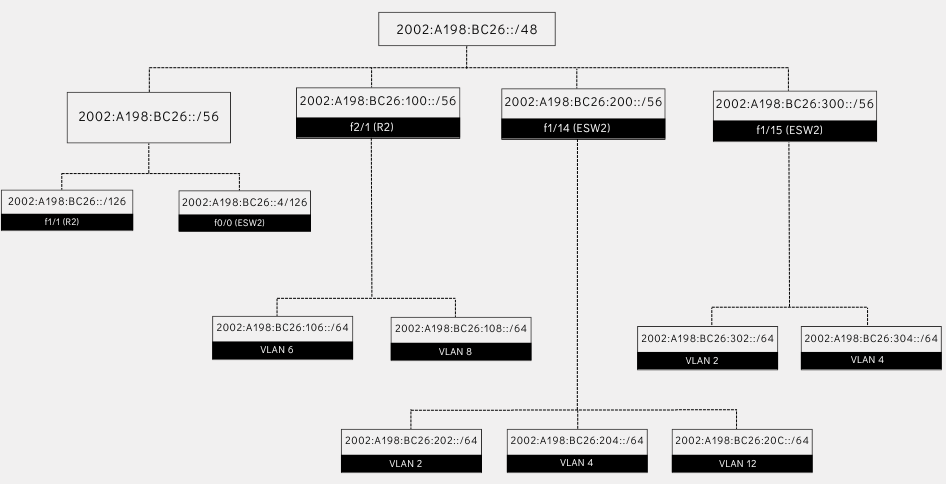
\includegraphics[width=20cm]{code/images/ipv6_global_calendar.png}
   % \caption{Legenda da imagem, se desejar} % Opcional
\end{figure}

\newpage
\clearpage

\section*{Horoscope Inc}

%\begin{tabular}{|m{2cm}|m{1,3cm}|m{2,3cm}|m{5cm}|m{2,5cm}|m{1cm}|}

\begin{table}[h!]
    \hspace*{-4.0cm}
    \centering
    \setlength{\tabcolsep}{2pt} % Reduz o espaçamento entre colunas
    \renewcommand{\arraystretch}{1.3} % Aumenta o espaçamento entre linhas
    \begin{tabular}{|c|c|c|c|c|c|} % Reduz a largura do campo Endereços Disponíveis
        \hline
        \textbf{Interface} & \textbf{Rede Interface} & \textbf{VLAN} & \textbf{Rede VLAN} & \textbf{Endereços Disponíveis} & \textbf{Default Gateway} \\ \hline
        
        \multirow{3}{*}{R1} & \multirow{3}{*}{\textbf{P}::/56} & 14 & \textbf{P}:E::/64 & \textbf{P}:E::2/64 a \textbf{P}:E:FFFF:FFFF:FFFF:FFFF/64 & \textbf{P}:E::1/64 \\ \cline{3-6} 
         & & 16 & \textbf{P}:10::/64 & \textbf{P}:10::2/64 a \textbf{P}:10:FFFF:FFFF:FFFF:FFFF/64 & \textbf{P}:10::1/64 \\ \cline{3-6}   
         & & 24 & \textbf{P}:18::/64 & \textbf{P}:18::2/64 a \textbf{P}:18:FFFF:FFFF:FFFF:FFFF/64 & \textbf{P}:18::1/64 \\ \hline

         R1 (f1/0) & \textbf{P}::1/126 & --- & --- & --- & --- \\ \hline

         ESW1 (f0/0) & \textbf{P}::2/126 & --- & --- & --- & --- \\ \hline
         
         \multirow{3}{*}{ESW1} & \multirow{3}{*}{\textbf{P}:100::/56} & 18 & \textbf{P}:112::/64 & \textbf{P}:112::2/64 a \textbf{P}:112:FFFF:FFFF:FFFF:FFFF/64 & \textbf{P}:112::1/64 \\ \cline{3-6}   
         & & 20 & \textbf{P}:114::/64 & \textbf{P}:114::2/64 a \textbf{P}:114:FFFF:FFFF:FFFF:FFFF/64 & \textbf{P}:114::1/64 \\ \cline{3-6}   
         & & 22 & \textbf{P}:116::/64 & \textbf{P}:116::2/64 a \textbf{P}:116:FFFF:FFFF:FFFF:FFFF/64 & \textbf{P}:116::1/64 \\ \hline

    \end{tabular}
    \textbf{Prefix (P):} 2002:A125:BC91
    \caption{Atribuição do IPv6 Global para Horoscope Inc}
\end{table}

Tendo a rede IP 2002:A125:BC91::/48, dividiu-se arbitráriamente por 2 redes IP com máscara /56, sendo estas: 
\begin{itemize}
    \item 2002:A125:BC91::/56;
    \item 2002:A125:BC91:100::/56; 
\end{itemize}

Posteriormente pegou-se na rede 2002:A125:BC91::/56 e dividimo-la em 3, atribuido o endereço 2002:A125:BC91:E::/64 à VLAN 14, o 2002:A125:BC91:10::/64 à VLAN 8 e o 2002:A125:BC91:18::/64, escolhendo arbitrariamente.

De seguida, e obtida a partir da rede 2002:A125:BC91::/48, obtivemos as seguintes sub-redes para a comunicação entre o Router 1 e o ESW 1:
\begin{itemize}
    \item 2002:A125:BC91::1/126;
    \item 2002:A125:BC91::2/126.
\end{itemize}

Por fim pegamos na rede 2002:A125:BC91:100::/56 e subdividimo-la em 3, atribuindo 2002:A125:BC91:112::/64 à VLAN 18, 2002:A125:BC91:114::/64 à VLAN 20 e 2002:A125:BC91:116::/64 à VLAN 22.

\newpage
\begin{figure}[H]
    \hspace*{-4.0cm}
    \centering
    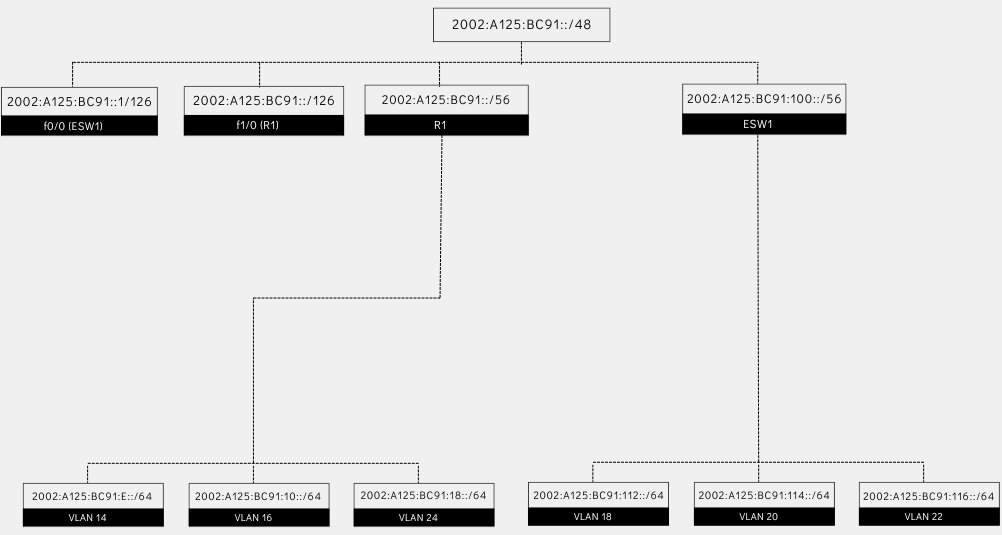
\includegraphics[width=20cm]{code/images/Horoscope Inc - IPv6.png}
   % \caption{Legenda da imagem, se desejar} % Opcional
\end{figure}

\newpage
\clearpage

\section*{\centerline {Atribuição de endereços IP}}
\begin{center}
\begin{tabular}{|c|c|c|c|}
    \hline
    \textbf{Terminal} & \textbf{VLAN id} & \textbf{Private IPv4} & \textbf{Public IPv4}\\ \hline
    January  & 2 & 172.26.12.2/24 & --- \\ \hline
    February & 2 & DHCP & ---  \\ \hline
    March  & 2 & --- & 203.128.191.164/28 \\ \hline
    April  & 4 & 172.26.13.130/25 & --- \\ \hline
    May & 4 & DHCP & --- \\ \hline
    June & 4 & --- & 203.128.191.132/27 \\ \hline
    July & 6 & 172.26.13.2/26 & --- \\ \hline
    August & 6 & DHCP & --- \\ \hline
    September & 6 & --- & 203.128.191.196/26 \\ \hline
    October & 8 & 172.26.13.98/27 & ---  \\ \hline
    November & 8 & DHCP & --- \\ \hline
    December & 8 & --- & 203.128.191.180/29 \\ \hline
    Calendar (VM) & 12 & --- & 203.128.191.190/30 \\ \hline
    ESW2 (f0/0) & --- & 172.26.13.65/30 & ---  \\ \hline
    R2 (f1/1) & --- & 172.26.13.66/30 & --- \\ \hline
    Aires & 14 & DHCP & --- \\ \hline
    Taurus & 14 & --- & 203.12.59.3/27 \\ \hline
    Gemini & 16 & 172.22.13.194/26 & --- \\ \hline
    Cancer & 16 & DHCP & --- \\ \hline
    Leo & 16 & --- & 203.12.59.100/27 \\ \hline
    Virgo & 18 & 172.22.13.2/26 & --- \\ \hline
    Libra & 18 & DHCP & --- \\ \hline
    Scorpius & 20 & 172.22.13.98/28 & --- \\ \hline
    Sagittarius & 20 & DHCP & --- \\ \hline
    Capricornus & 22 & --- & 203.12.59.50/29  \\ \hline
    Aquarius & 20 & --- & 203.12.59.84/28 \\ \hline
    Pisces & 18 & --- & 203.12.59.36/28 \\ \hline
    Horoscope (VM) & 24 & --- & 203.12.59.62/30 \\ \hline
    R1 (f1/0) & --- & 172.22.13.113/30 & --- \\ \hline
    ESW1 (f0/0) & --- & 172.22.13.114/30 & --- \\ \hline
\end{tabular}
\end{center}


%%%%%%%%%%%%%%%%%%%%%%%%%%%%%%%%%
\printbibliography

\end{document}